\newcommand{\novp}{\textit{\textbf{NoVP}}}
\newcommand{\vp}{\textit{\textbf{VP}}}
\newcommand{\nfnovp}{\textit{\textbf{RFNoVP}}}
\newcommand{\nfvp}{\textit{\textbf{RFVP}}}

\newcommand{\optvp}{\textit{\textbf{OptVP}}}
\newcommand{\vt}{\textit{\textbf{VT}}}
\newcommand{\nfvt}{\textit{\textbf{RFVT}}}
\subsection{Setup}
This chapter demonstrates that modifying the hardware to improve the performance of core composition requires the implementation of complex systems.
The modifications discussed in the chapter are better branch prediction, adding a value predictor, and modifying the block fetching scheme.
Whilst a value predictor improves performance by allowing blocks to execute independently via speculating register values, value predictors are still considered a work in progress~\cite{peraisBeBop2015}.
It is important to consider how a perfect system with the new hardware additions can improve the performance of core composition, as it gives an upper bound to the potential performance increases.

This section therefore explores how a perfect branch and value predictor, paired with the new fetching scheme, improves the performance of core composition on the SD-VBS benchmarks.
To understand how each component contributes to the performance improvements, different configurations were used, they are as follows:
\begin{itemize}
\item Normal fetching scheme with no value prediction (\novp).
\vspace{-1em}
\item Normal fetching scheme with perfect value prediction (\vp).
\vspace{-1em}
\item New fetching scheme with no value prediction (\nfnovp).
\vspace{-1em}
\item New fetching scheme with value prediction (\nfvp).
\end{itemize}

\begin{figure}[t]
    \centering
    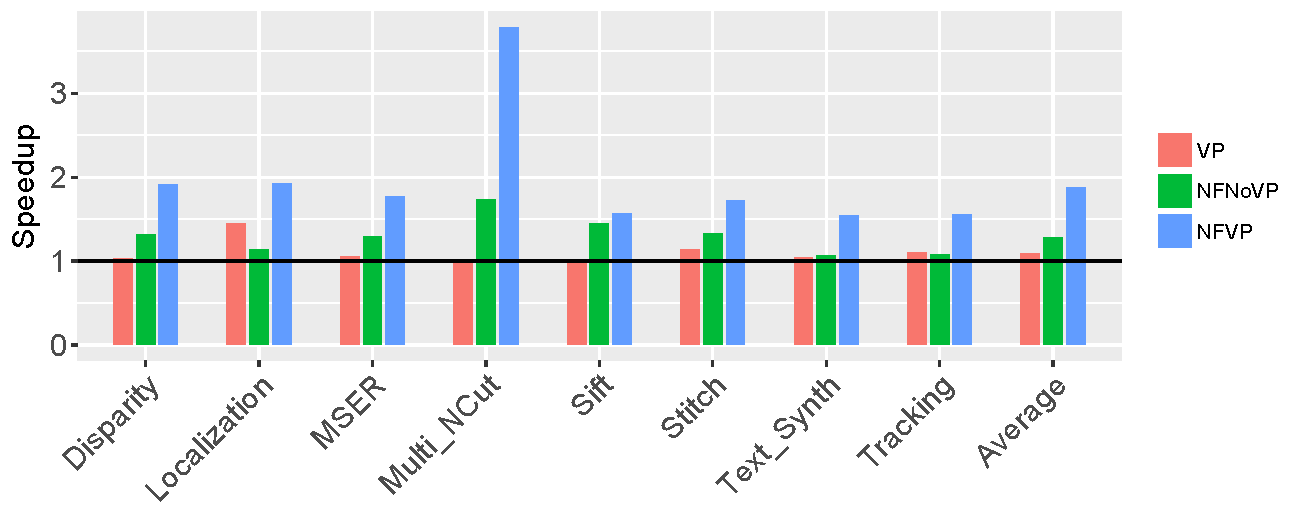
\includegraphics[width=1\textwidth]{chapter3/graphics/tempres2.pdf}
    \caption{Comparing the performance of the standard fetching scheme to the new fetching scheme, with and without perfect value prediction. Higher is better}
    \label{fig:perf_pred}
\end{figure}
All configurations use perfect branch prediction as to ensure that core composition is always on the correct execution path.

\subsection{Results}
Figure~\ref{fig:perf_pred} shows the speedup obtained on the SD-VBS benchmarks using the different configurations.
The baseline for this section is normal fetching scheme with no value prediction (\novp).
It is chosen as it represents a setup similar to the previous two chapters, the only difference being the perfrect branch prediction.
The number of cores composed for each benchmark using the different configurations can be found in Table~\ref{tab:conf_cores}.
As this chapter is primarily interested in getting the fastest execution times, only the fastest core composition is shown in the results.

\begin{table}[t]
  \small
  \centering
 \begin{tabular} {| l | l | l | l | l | l | }
 \hline
    & \cellcolor[gray]{0.7}Disparity & \cellcolor[gray]{0.7} Localization& \cellcolor[gray]{0.7} MSER& \cellcolor[gray]{0.7} Multi\_NCut& \cellcolor[gray]{0.7} Sift\\ \hline
 \novp   & 16  & 16 & 4  & 16& 16\\ \hline
 \vp   & 16  & 16 & 4  & 16& 16\\ \hline
 \nfnovp   & 16  & 16 & 4  & 16& 16\\ \hline
 \nfvp   & 16  & 16 & 4  & 16& 16\\ \hline
	  & \cellcolor[gray]{0.7} Stitch & \cellcolor[gray]{0.7} SVM & \cellcolor[gray]{0.7} Text. Synth & \cellcolor[gray]{0.7} Tracking&\\ \hline
\novp	 & 16& 16& 16& 16 &\\ \hline
   \vp & 16  & 16 & 4  & 16 & \\ \hline
 \nfnovp  & 16  & 16 & 4  & 16 & \\ \hline
 \nfvp   & 16  & 16 & 4  & 16 &\\ \hline

	\end{tabular}
  \caption{Number of cores composed given a configuration.}\label{tab:conf_cores}
  \vspace{1em}
\end{table}

First, it is clear that using the new fetching scheme with value prediction (\nfvp) always results in the best speedup compared to the baseline.
For \bm{Multi\_NCut}, performance is improved by almost 4x when using \nfvp.
This is a significant speedup, as Chapter~\ref{chp:cases} showed that \bm{Multi\_Ncut} was a difficult benchmark for core composition.
On average, \nfvp{} outperforms the baseline by a factor of 1.88x.

The results in Figure~\ref{fig:perf_pred} show that when the new fetching scheme is not paired with value prediction, the performance improvements are less important.
For example, \bm{Localization} only has a 1.10x speedup when using the \nfnovp{} configuration, compared to the 1.90x of \nfvp{}.
This is due to the fact that whilst blocks are fetched faster, the register dependencies between blocks limit the performance of core composition.
The performance limitations are caused by blocks that are further down the speculative that must wait for older blocks to write to the register file.
In fact, \vp{} outperforms \nfnovp{} on \bm{Localization}, which shows that register dependencies between blocks can make the new fetching scheme less performant than the currently implemented.

On the other hand, \bm{Multi\_NCut} with \textbf{\textit{NFNoVP}} has a 1.60x speedup compared to the baseline.
This is because \bm{Multi\_NCut} has small blocks, on average less than 10 instructions long as seen in Chapter~\ref{chp:cases} Section~\ref{sec:expl}.
When blocks are uniformly small, value prediction will not help when using the normal fetching scheme, as the composition will never be full, thus explaining why \vp{} does not perform better than the baseline.

The performance of \vp{} compared to \novp{} can be surprising as the perfect value prediction does not appear to speed up execution.
Value prediction is most useful when multiple data-dependent blocks are in flight as the data can be speculated.
However, as seen in Section~\ref{chp3:sec:fetch} the normal fetching scheme is too slow to ensure that all cores in a composition are executing blocks.
Therefore, value prediction does not benefit baseline setup, as the large core compositions are never full.

\begin{figure}[t]
    \centering
    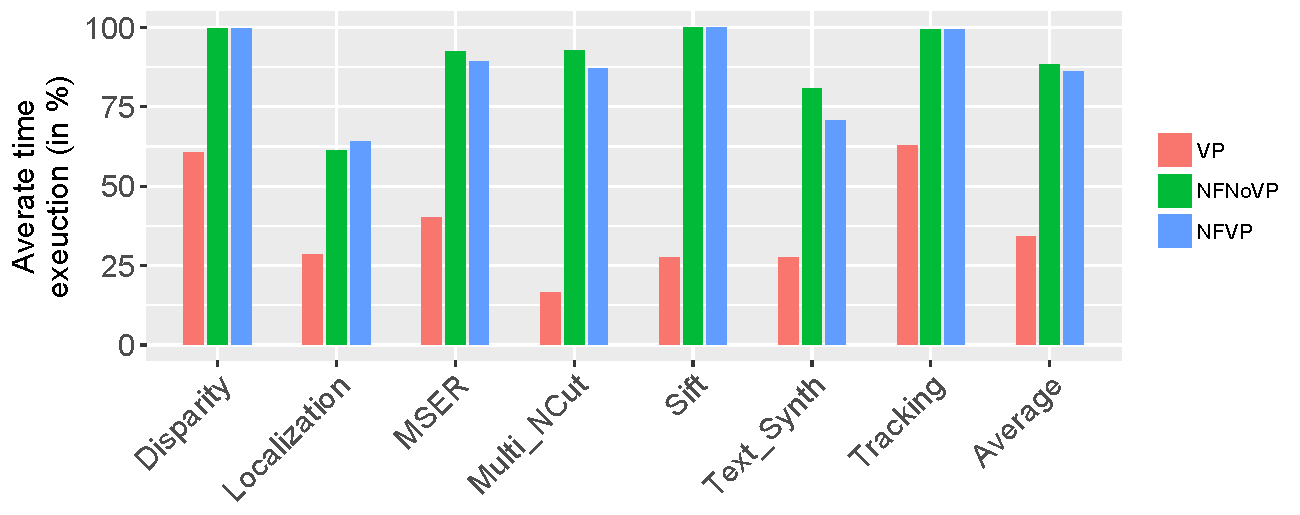
\includegraphics[width=1\textwidth]{chapter3/graphics/perf_av_cycle_exec2.pdf}
    \caption{Average time each core is executing blocks (in \%) for each benchmark, using the different configurations. Higher is better.}
    \label{fig:perf_av_cycle}
	\vspace{1em}
\end{figure}

To better highlight how the normal fetching scheme hinders performance even with value prediction, the percentage of time a core in a composition was actively executing code, for each benchmark, is shown in Figure~\ref{fig:perf_av_cycle}.
For each configuration, the number of cycles each core in a composition executed instructions is averaged out and then compared to the total execution time of the application.
When the average active time of a core is close to the total execution time, this means that the composition was efficiently used, as each core executed the same amount of code.

As Figure~\ref{fig:perf_av_cycle} shows, \novp{} and \vp{} often have low active time percentages.
This is due to the fact that the current serialised block fetching scheme is slow, and thus, some cores will be innactive, waiting to receive a fetch request from another core.
The lower the percentage is, the less likely there are going to be multiple blocks on different cores in flight which in turn means value prediction is less useful.
The reason \novp{} has a higher average time of execution than \vp{} is due to the fact that in cases where value prediction is in fact usefull, it reduces the execution time of blocks.
If block execution time is reduced, this decreases the opportunity for efficient use of large core compositions due to how the fetching mechanism is slow (recall Figure~\ref{fig:new_fetch_ex} in Section~\ref{chp3:sec:fetch}).
Since value prediction is aimed at increasing instruction level parallelism (ILP)~\cite{peraisBeBop2015} it is important that cores may fetch blocks quickly in a composition.
The lack of performance differences between \novp{} and \vp{} is proof that a faster fetching scheme is required to allow core composition to benefit from value prediction.

With the new fetching scheme, the percentage of active time is increased on average by a factor of 2.28x, and is on average 85\%.
This means that during most of the execution of an application, all cores are executing code, and thus greatly increases the chance of improving performance via core composition.
Interestingly enough, whilst the new fetching scheme aims to evenly distribute blocks amongst the cores, the average core utilisation for \bm{Localization} with the configurations \nfnovp{} and \nfvp{} is of 62\%.

\begin{figure}[t]
    \centering
    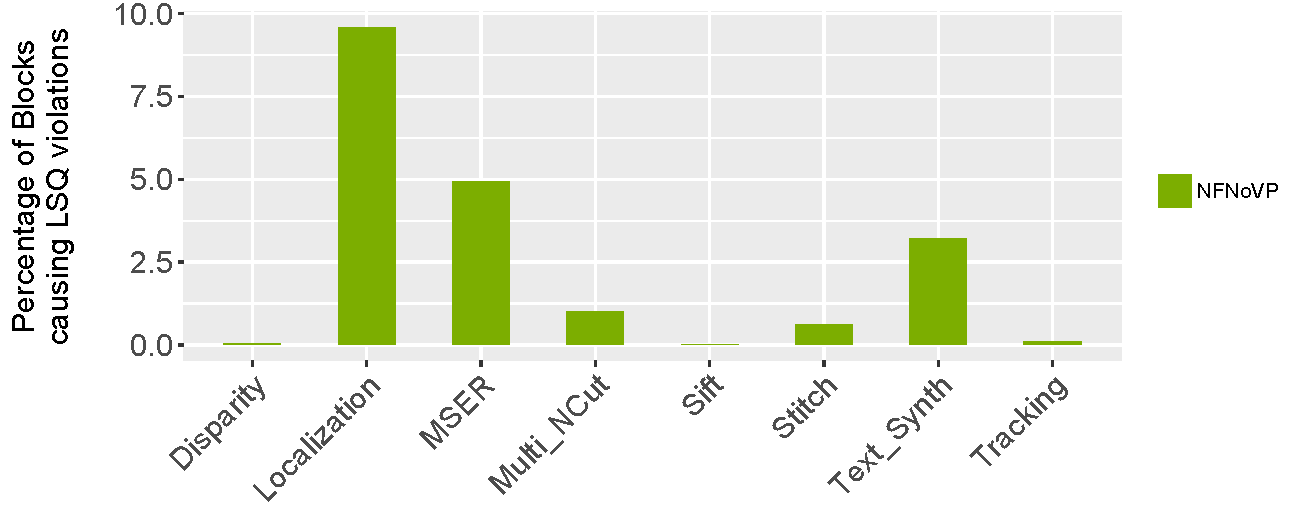
\includegraphics[width=1\textwidth]{chapter3/graphics/lsqViol2.pdf}
    \caption{Number of blocks that cause LSQ violations, normalised by the number of committed blocks for each of the benchmarks.}
    \label{fig:lsqvio}
	\vspace{1em}
\end{figure}

This is due to flushes caused by Load-Store-Queue (LSQ) order violations, which causes cores to flush their instruction windows, and thus increases the number of times that cores will not be executing code.
Figure~\ref{fig:lsqvio} shows the number of blocks that cause an LSQ violation, normalized by the number of committed blocks for each of the benchmarks.
In this graph, 10\% of fetched blocks caused an LSQ violation, this is twice as much as the second benchmark impacted by violations (\bm{MSER}).
A store-set dependency predictor is implemented in the processor, however it is sometimes hard to predict load-store dependencies accross multiple blocks, thus causing LSQ dependency violations.
Store-set dependency predictors are not discussed in more detail in this chapter, however researching how store-set dependencies could be applied to core-composition is an interesting subject for future work.

\subsubsection{New fetching scheme bottleneck Analysis}

As seen in the previous section the new fetching scheme enables better use of the perfect value predictor. 
Whilst \nfnovp{} can improve performance by up to 2x as seen in \bm{Multi\_NCut} on average it only obtains a speedup of 1.27x compared to \novp{}.
This section covers where the bottlenecks of the new fetching scheme are found, what potential solutions can be employed, and how that can improve performance overall.

\paragraph*{Block fetching latency}

The new fetching scheme improves performance of a core composition by reducing the amount of communication between cores.
This is achieved through a pipeline-model fetching scheme, where cores do not fetch blocks sequentially, but rather in strides.
This does introduce one extra complexity: blocks that are further down the speculative path may be fetched before blocks closer to the non-speculative block.
To avoid any potential inconsistencies that may arise from dispatching blocks out of order, a block must wait for its parent block to be dispatched.

\begin{figure}[t]
    \centering
    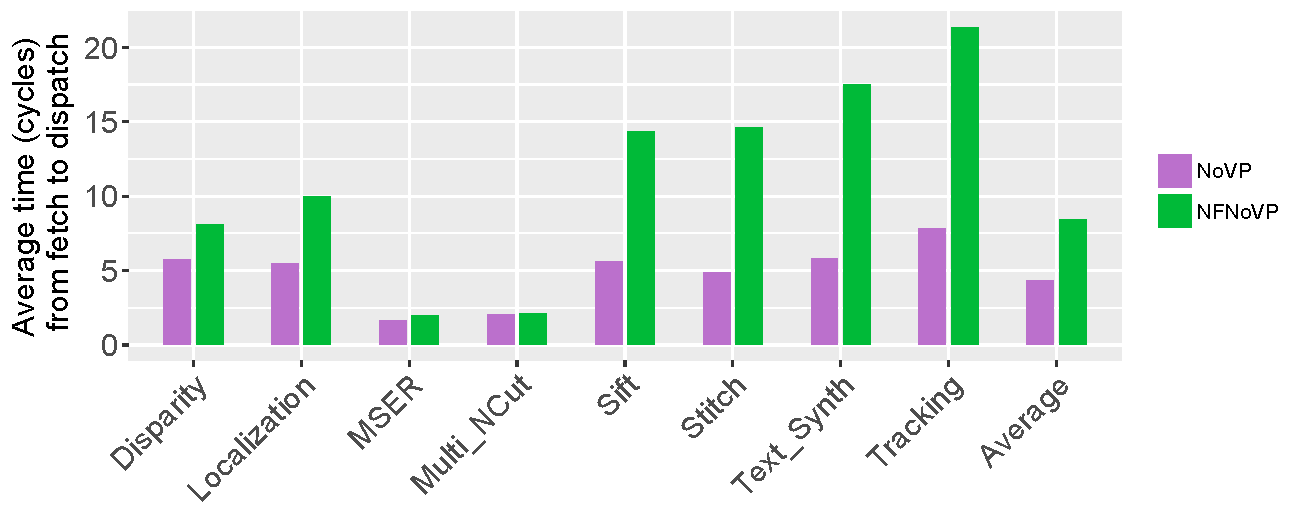
\includegraphics[width=1\textwidth]{chapter3/graphics/avTimeToFetch2.pdf}
    \caption{Average time (in cycles) for block to go from fetched to dispatched using the current fetching scheme and new fetching scheme. Lower is better.}
    \label{fig:av_time}
	\vspace{1em}
\end{figure}

This means that cores may have fetched blocks in their window that must wait a certain number of cycles before executing.
To understand how this affects the performance of the new fetching scheme, the average time from a block being fetched, to a block being dispatched is recorded in the simulator.
Comparing the average time between the current and new fetching scheme can provide an estimate as to how much performance is potentially lost in the new fetching scheme.

Figure~\ref{fig:av_time} shows the average time for all the SD-VBS benchmarks using the current and new fetching scheme.
As can be seen, for most benchmarks, the new fetching scheme's average time is 2x slower than the current.
This is due to the fact that whenever the current fetching scheme fetches a block, it can immediately dispatched as fetches are serialised.
\bm{Multi\_Ncut} has the lowest difference, which explains why it obtains the highest speedup with \nfnovp{}.
It is important to note that \bm{MSER} and \bm{Multi\_Ncut} have lower average times than all other benchmarks as their blocks are mostly small and thus quick to dispatch.
Even with the extra latency, the new fetching scheme still ensures that every core is full, cores must now only wait for their blocks to be dispatched, rather than having for a fetch request.

%Explain how different blcok sizes may mess up the new fetching scheme

\begin{figure}[t]
    \centering
    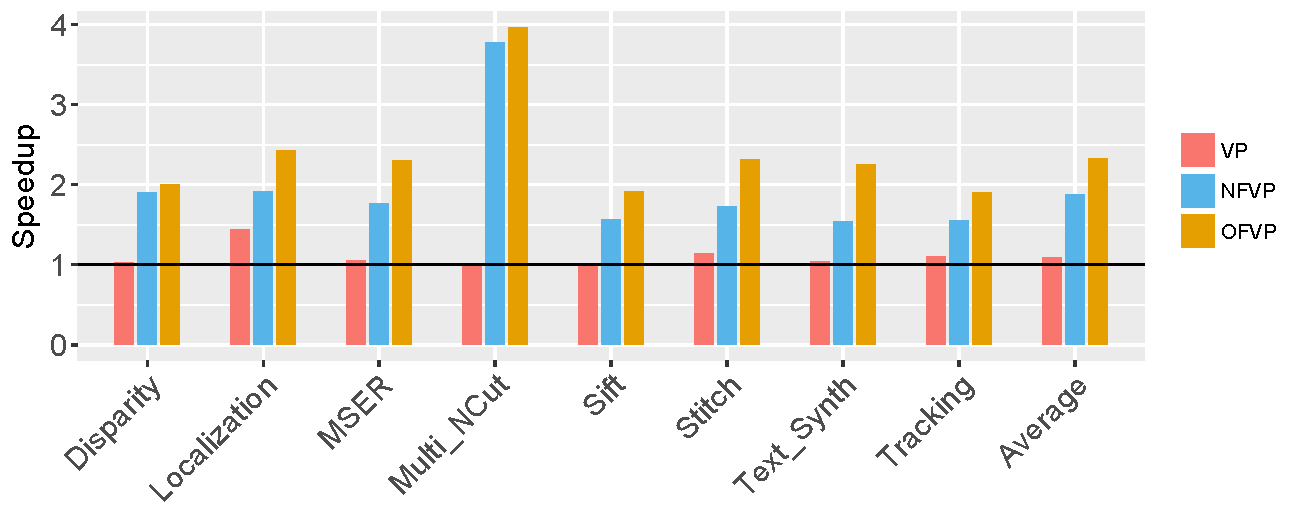
\includegraphics[width=1\textwidth]{chapter3/graphics/opt_res2.pdf}
    \caption{Comparing the performance of an optimal fetching scheme with \vp{} and \nfvp{}, baseline is \novp. Higher is better.}
    \label{fig:opt_scheme}
	\vspace{1em}
\end{figure}

\paragraph*{Enhancing the new fetching scheme}

The new fetching scheme aims to decentralise block fetches by statically determining the stride at which a core fetches ahead of time.
As Figure~\ref{fig:av_time} shows, this increases the average time between a core fetching a block and dispatching it as cores may fetch blocks too far into the speculative chain.
This increase in average time is due to cores fetching blocks that are too far into the speculative chain due to the fixed fetch stride.
Relaxing the new fetching scheme by allowing cores to fetch any block can potentially improve performance.

To understand how much this added time between fetch and dispatch impacts performance, the total number of cycles a core must wait before dispatching a block is recorded for the new fetching scheme.
Once the program has terminated, this number is averaged out by the number of cores in the composition and subtracted from the total cycle count.
This optimistically emulates a perfect fetching scheme in which cores fetch blocks in parallel and can immediately dispatch them in order, this configuration is named Optimal Fetching with Value Prediction (\optvp).

Figure~\ref{fig:opt_scheme} shows how \optvp{} compares to \vp{} and \nfvp{}, with \novp{} as a baseline.
The graph shows that most applications benefit from \optvp{}, averaging at a speedup of 2.32x compared to \nfvp's 1.88x which is a 23\% increase.
This increase can be considered optimistic, however it shows that some modifications to the new fetching scheme can potentially improve performance further.

\subsubsection{Summary}

This section shows that a perfect branch predictor, paired with perfect value prediction and a new fetching scheme can outperform the current configuration by a factor of up to 4x.
On average, new configuration obtains a speedup of 1.88x, and can potentially be improved to 2.23x with further modifications to the fetching scheme.

